\chapter{Introduction}

\section{Introduction to Chromium project}
Following the Chromium Project official website \cite{chromium}, \textit{``Chromium is an open-source browser project that aims to build a safer, faster, and more stable way for all Internet users to experience the web"}. This project is the Open Source version of one of the most popular web browser nowadays, Google Chrome.

Chromium was released under a BSD license on 2008 \cite{release} by Google, at the same time that Chrome did. The purpose of the project was to distribute the source code of the Chrome browser, in order to enable third-party developers to study, modify, extend, and redistribute it. For the time being, following OpenHub charts, this project has more than 25 MLOC \footnote{Million Lines Of Code} and more than 9,000 commits per month. This commits are not only made by Google but for different organizations and independent developers. 

Even that this project integrates more than 30 languages, near the 50\% of the code is written in \texttt{C++}.


\section{Relationship with Google Chrome}

Although Chrome has more features than Chromium, Chromium provides the vast majority of source code for Google Chrome, including the user interface, the Blink rendering engine, and the V8 JavaScript engine. Thus Google chose the ``Chromium" name as an analogy of chromium metal forged into chrome plating.
\begin{figure}[H]
    \centering
    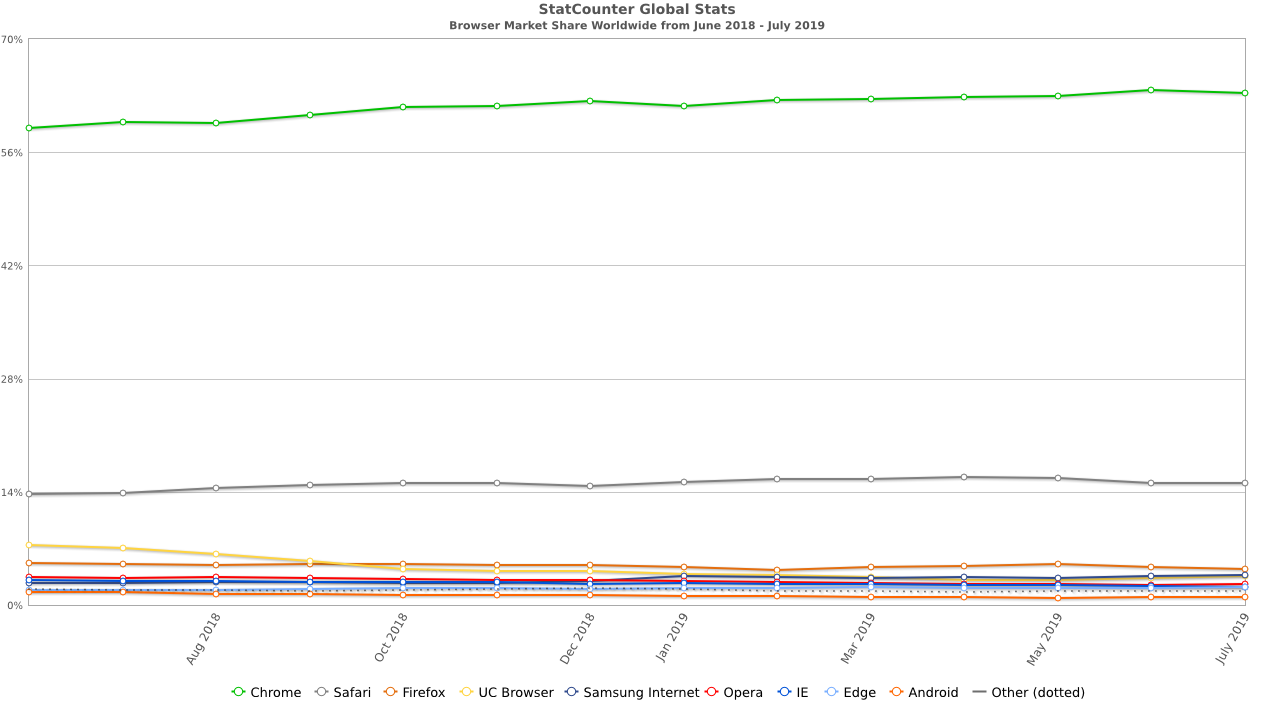
\includegraphics[width=\textwidth]{img/compare.png}
    \caption{Browser usage as of 2019}
    \label{fig:usage}
\end{figure}
As of 2019, StatCounter \cite{usage} (figure \ref{fig:usage}) estimates that Chrome has a 63\% worldwide browser market share across all platforms.


\section{Assignment goals}
The two main goals of the assignment are:

\begin{enumerate}
    \item Applying and contrasting all the knowledge acquired during the theoretical lectures and the invited talks to the study of a real, professional, complex open source project.
    \item Producing a report summarizing all the findings and derived proposals (i.e., this document).
\end{enumerate}


\section{Document structure}
From now on, this document is structured as follows:
\begin{description}
    \item[Chapter \ref{chap:methodology}] Aims to introduce the contribution policy and the technological tools used in the project.
    \item[Chapter \ref{chap:architecture}] We describe some technical aspects about Chromium's software architecture, delving in its multi-process characterization.
    \item[Chapter \ref{chap:design}] The IPC Component is analyzed and described. We also elaborated a set of UML diagrams that helped us to detect some software Design Patterns.
    \item[Chapter \ref{chap:quality}] The key concepts of quality are studied over the project in this chapter.
    \item[Chapter \ref{chap:accessibility}] We take a view on the main accessibility features of Chromium.
    \item[Chapter \ref{chap:interview}] A short but valuable interview with Julie Jeongeun Kim, a Chromium's developer, is presented.
    \item[Chapter \ref{chap:conclusions}] This essay ends with a short impression about what we learned during the analysis and discuss the possible lines of future work.
\end{description}